\subsection{The effect of particle dynamics model}

\begin{figure}[H]
	\centering
	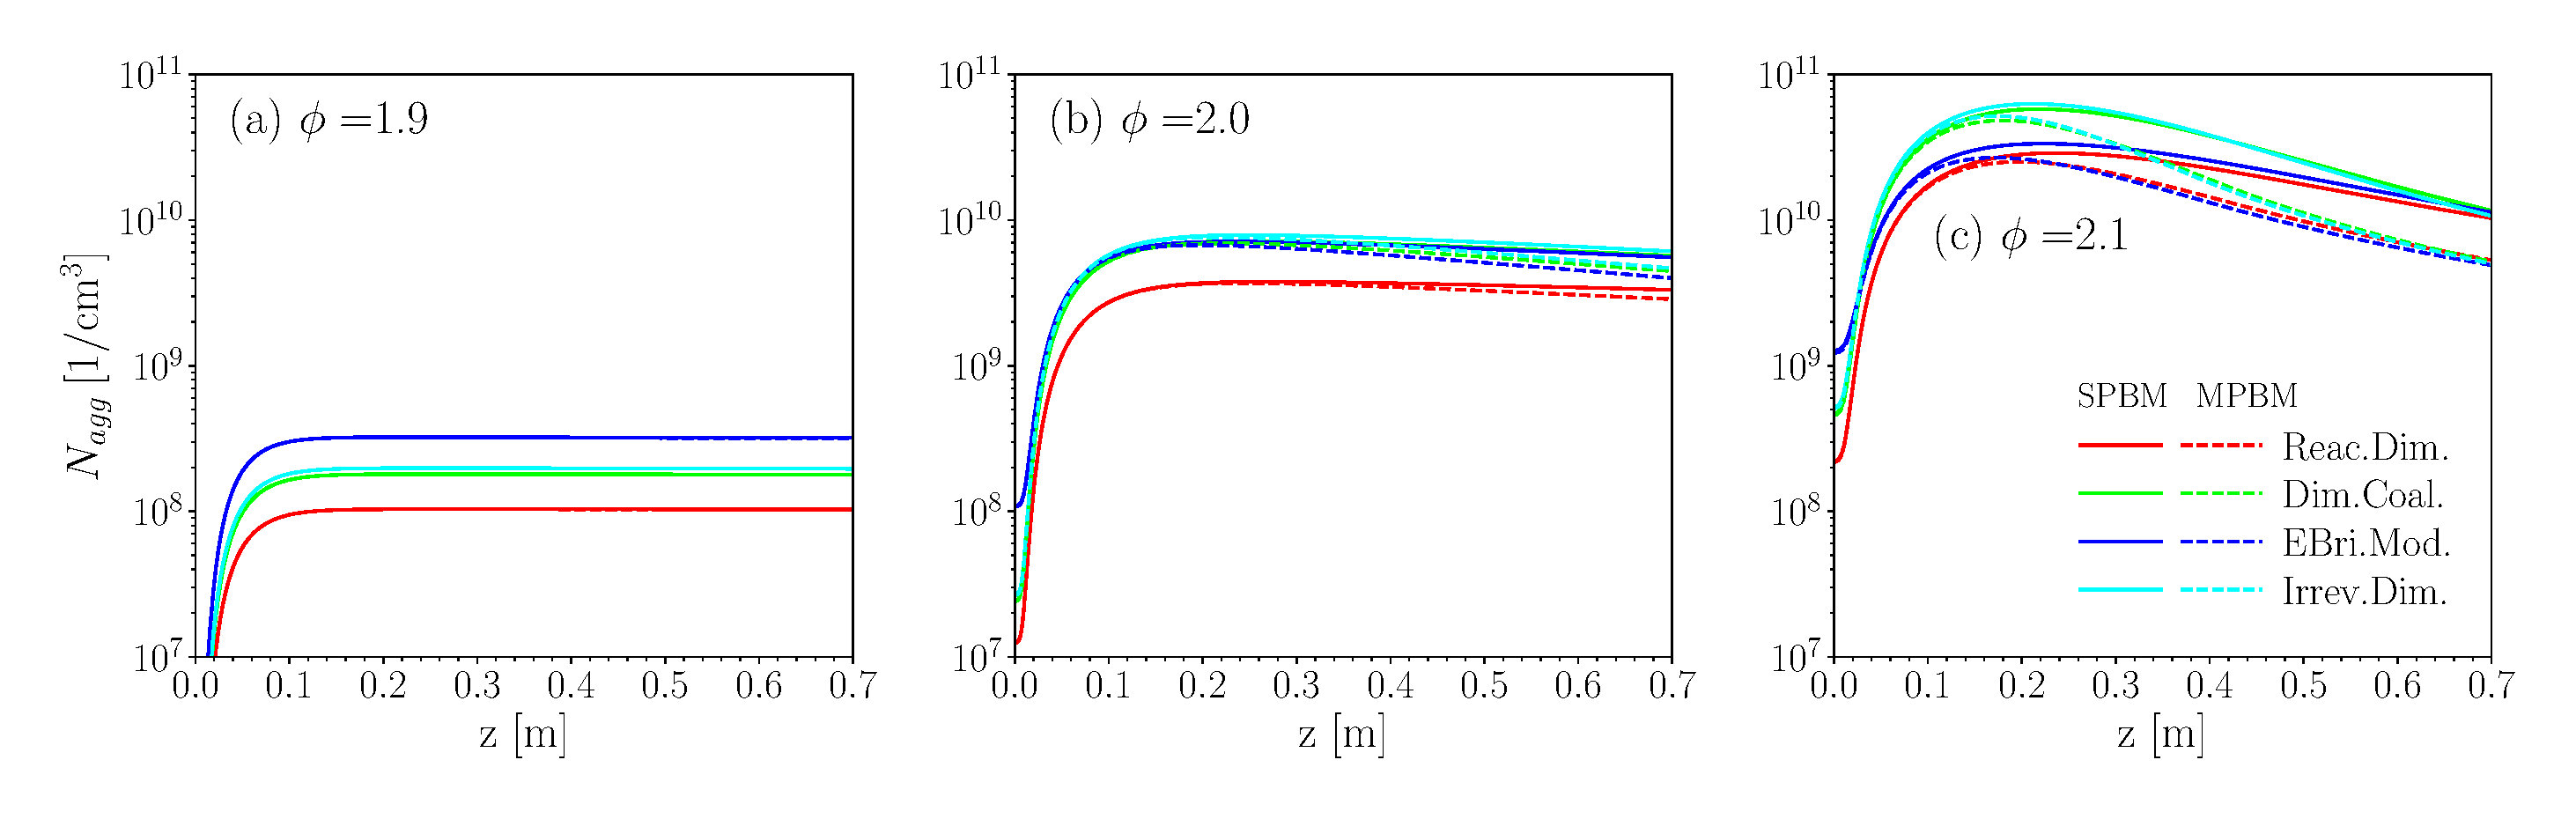
\includegraphics[width=1\textwidth]{Figures/Results/PSR/N_agg_eq_ratio_pdynamiceffect.pdf}
	\caption{The effect of particle dynamics on total number of agglomerates, $N_{agg}$ along the PFR in the downstream of a PSR~\citep{manzello2007soot} for $\phi$=1.9 (a), 2.0 (b), and 2.1 (c) obtained using KAUST mechanism and different inception models.}
	\label{fig:psr_Nagg_pdynamicseffect} 
\end{figure}

\begin{figure}[H]
	\centering
	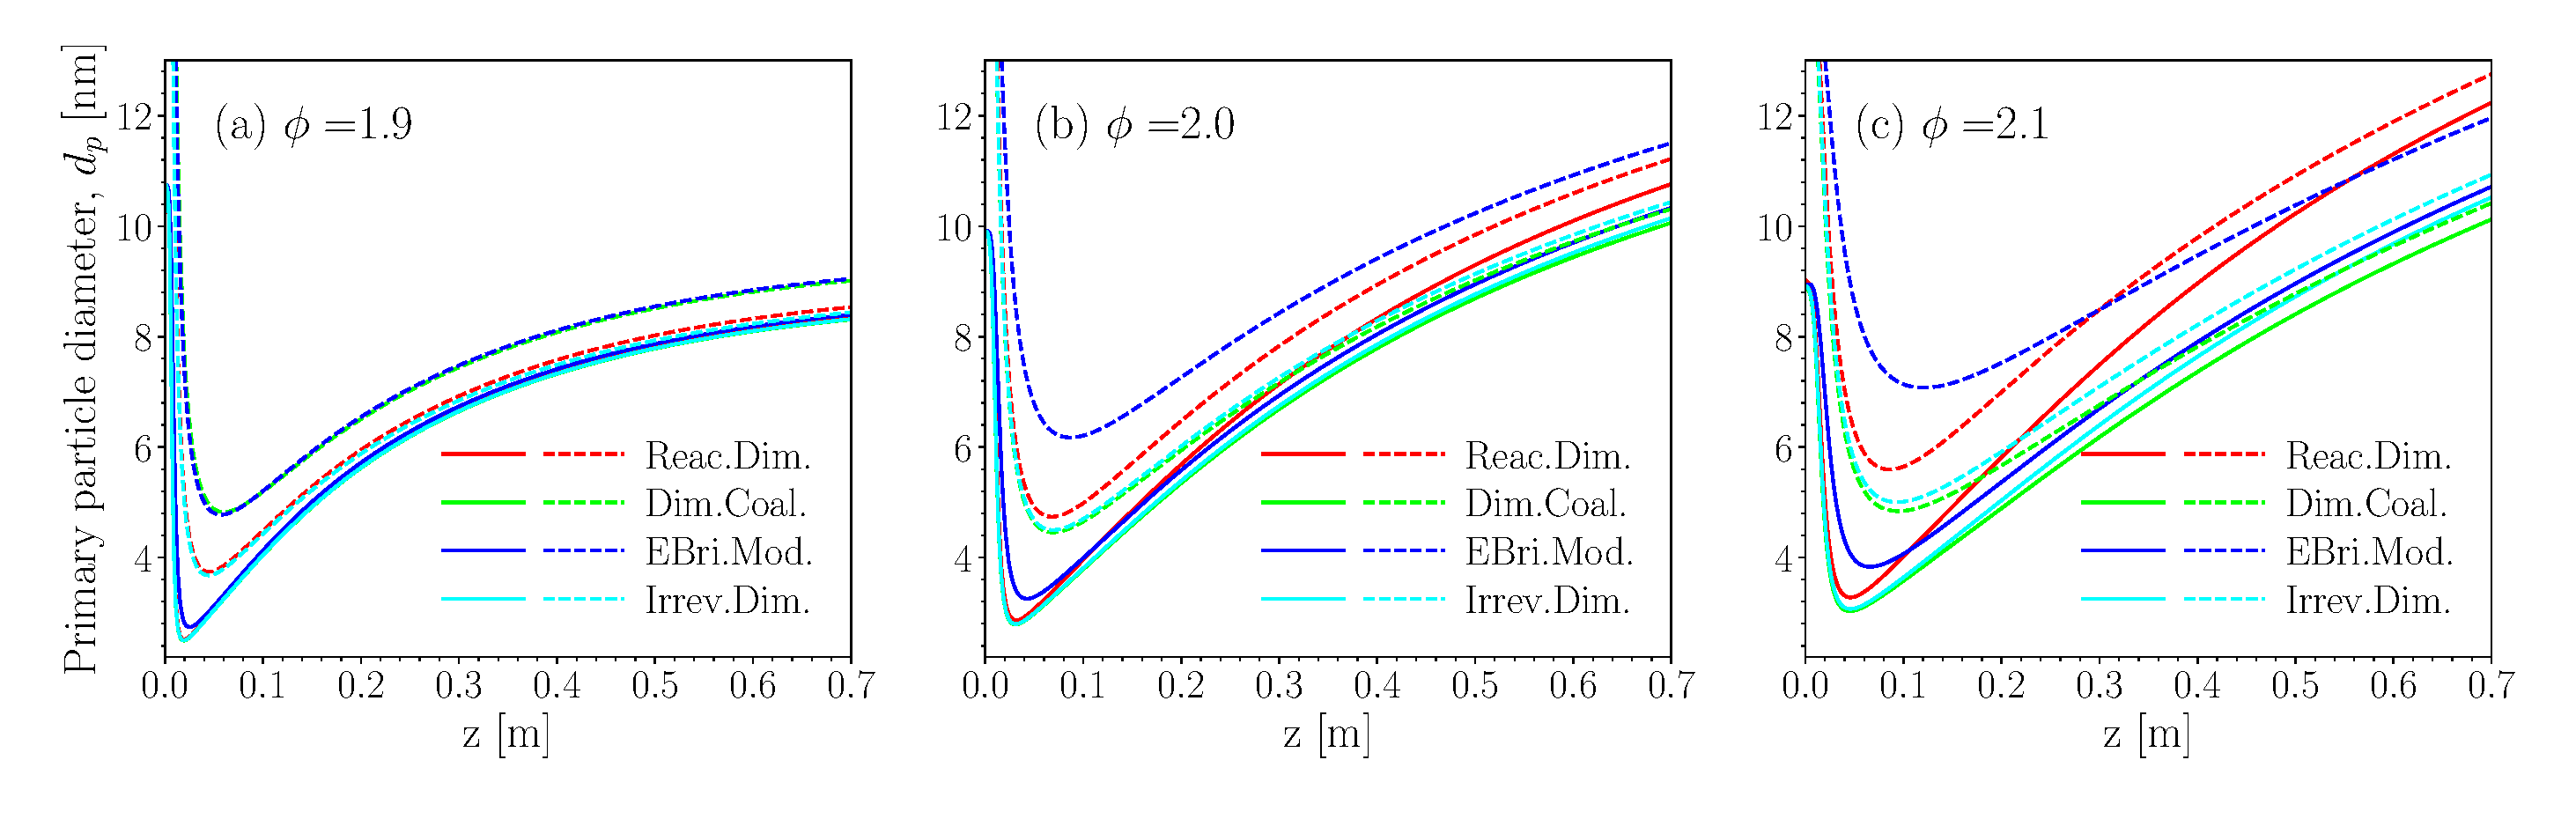
\includegraphics[width=1\textwidth]{Figures/Results/PSR/d_p_eq_ratio_pdynamiceffect.pdf}
	\caption{The effect of particle dynamics on primary particle diameter, $d_{p}$ along the PFR in the downstream of a PSR~\citep{manzello2007soot} for $\phi$=1.9 (a), 2.0 (b), and 2.1 (c) obtained using KAUST mechanism and different inception models.}
	\label{fig:psr_d_p_pdynamicseffect} 
\end{figure}


\begin{figure}[H]
	\centering
	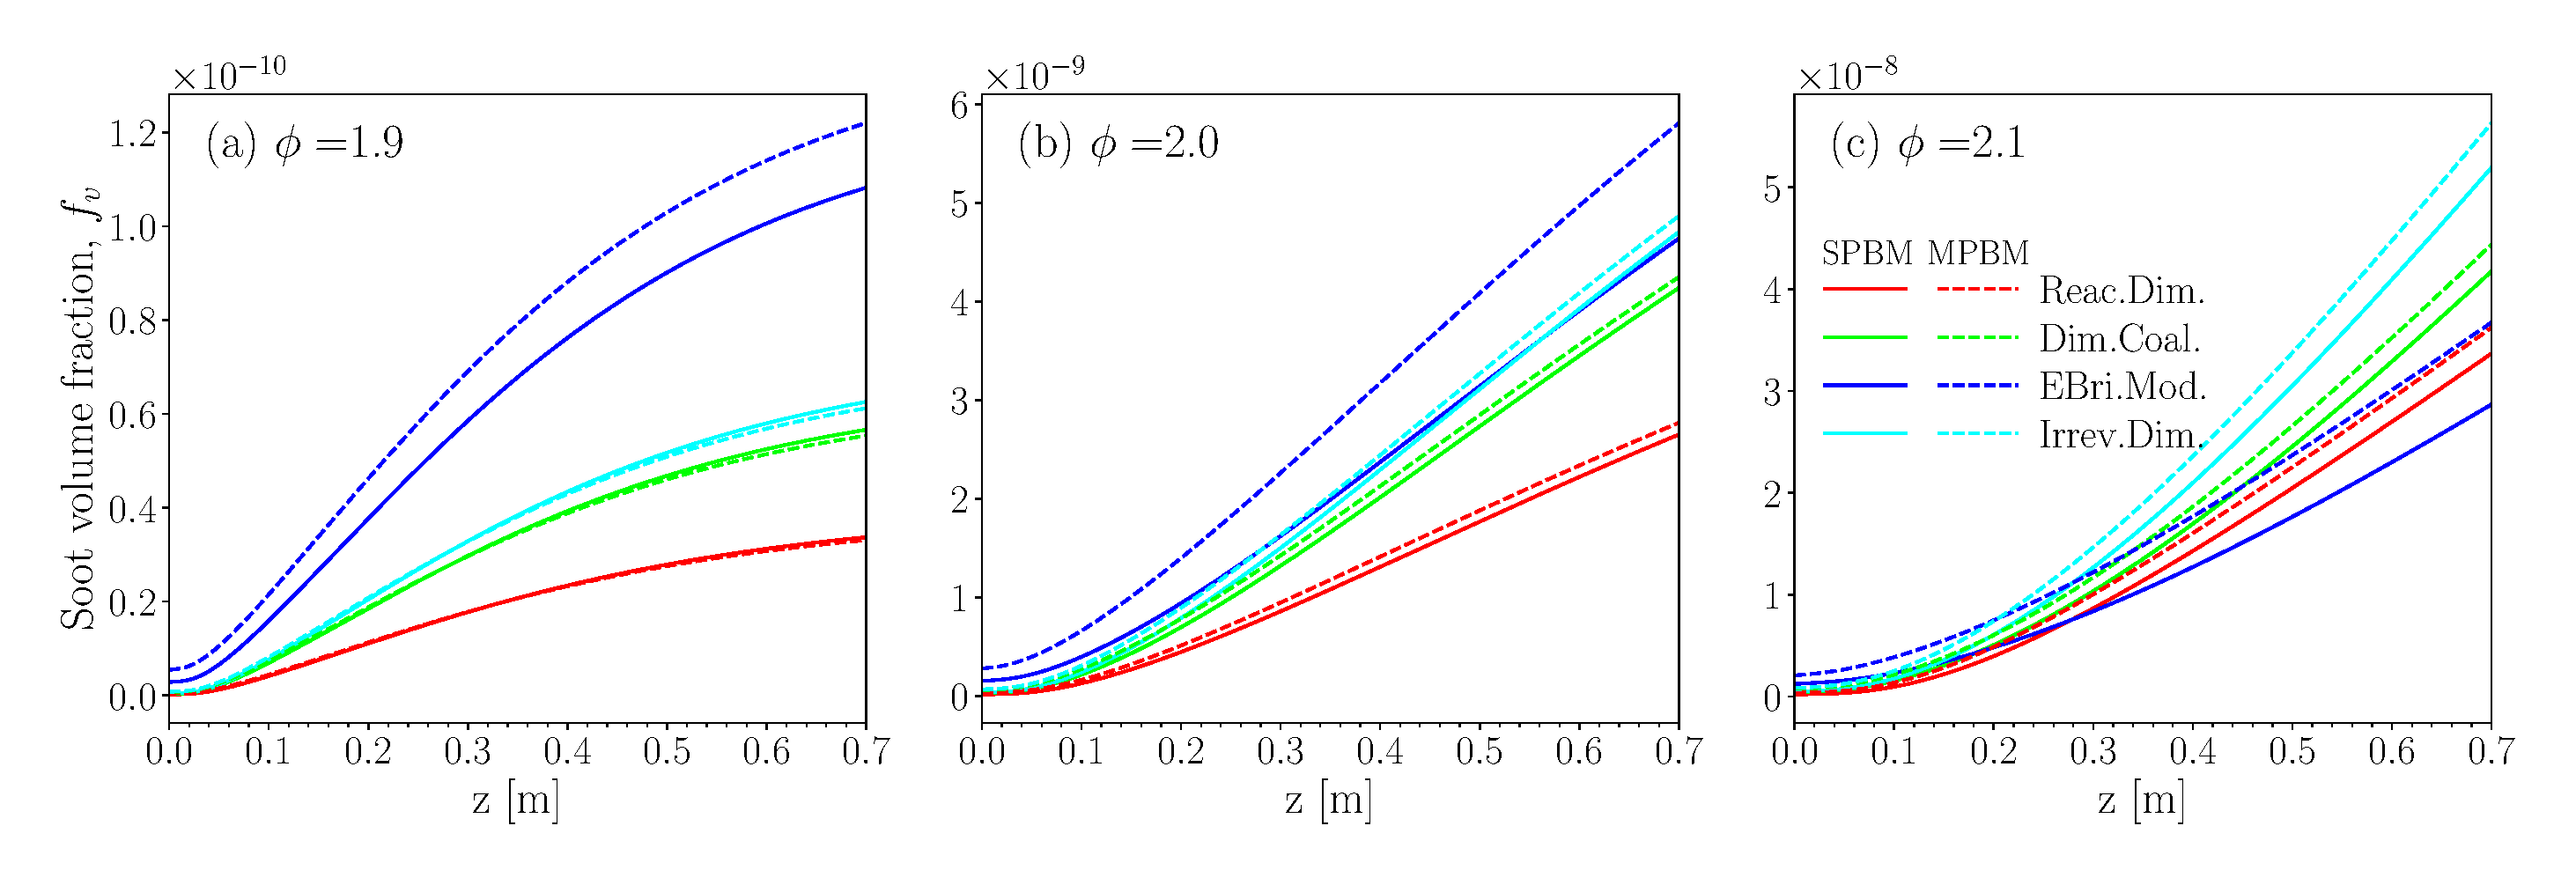
\includegraphics[width=1\textwidth]{Figures/Results/PSR/f_v_eq_ratio_pdynamiceffect.pdf}
	\caption{The effect of particle dynamics on soot volume fraction, $f_{v}$ along the PFR in the downstream of a PSR~\citep{manzello2007soot} for $\phi$=1.9 (a), 2.0 (b), and 2.1 (c) obtained using KAUST mechanism and different inception models.}
	\label{fig:psr_f_v_pdynamicseffect} 
\end{figure}

\begin{figure}[H]
	\centering
	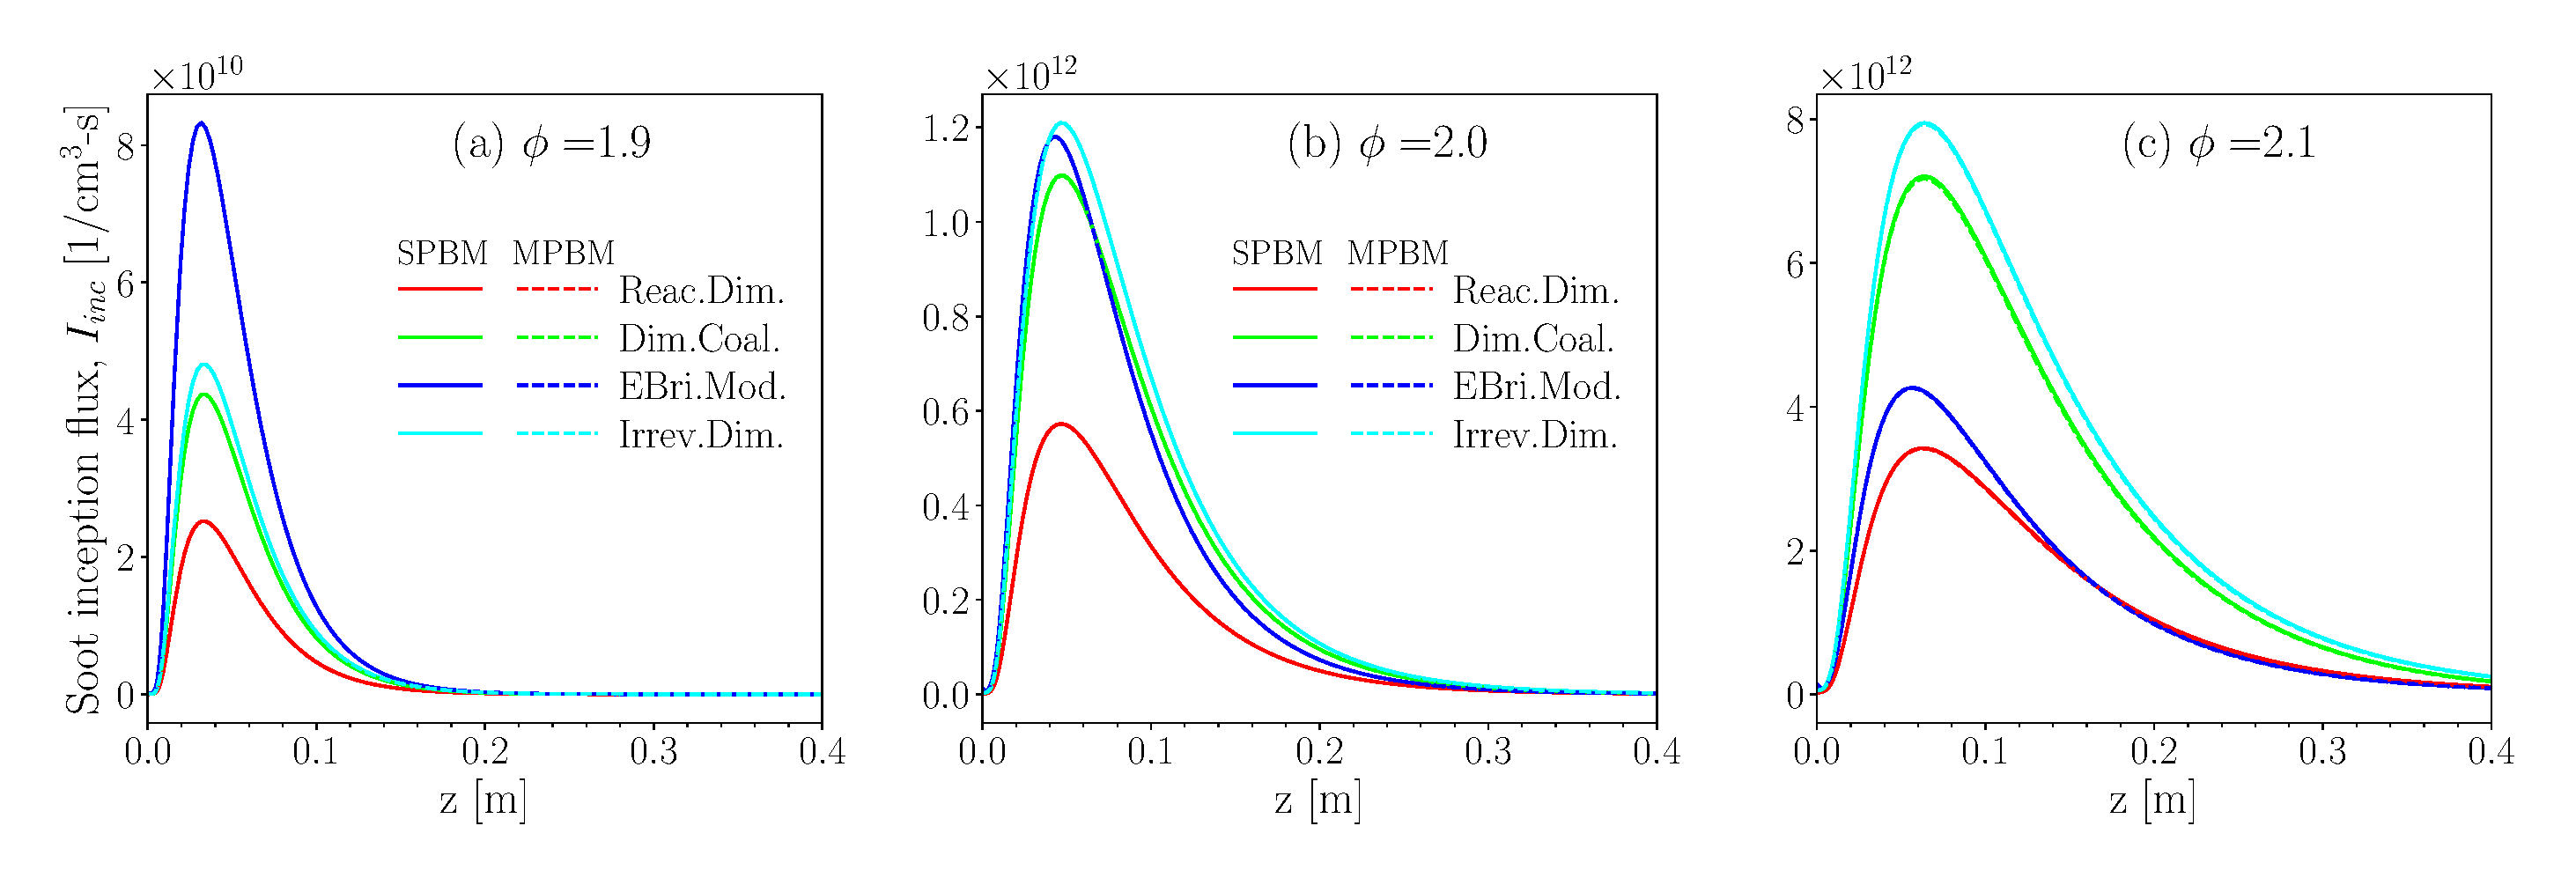
\includegraphics[width=1\textwidth]{Figures/Results/PSR/I_inc_eq_ratio_pdynamiceffect.pdf}
	\caption{The effect of particle dynamics on soot inception flux, $I_{inc}$ along the PFR in the downstream of a PSR~\citep{manzello2007soot} for $\phi$=1.9 (a), 2.0 (b), and 2.1 (c) obtained using KAUST mechanism and different inception models.}
	\label{fig:psr_I_inc_pdynamicseffect} 
\end{figure}


\begin{figure}[H]
	\centering
	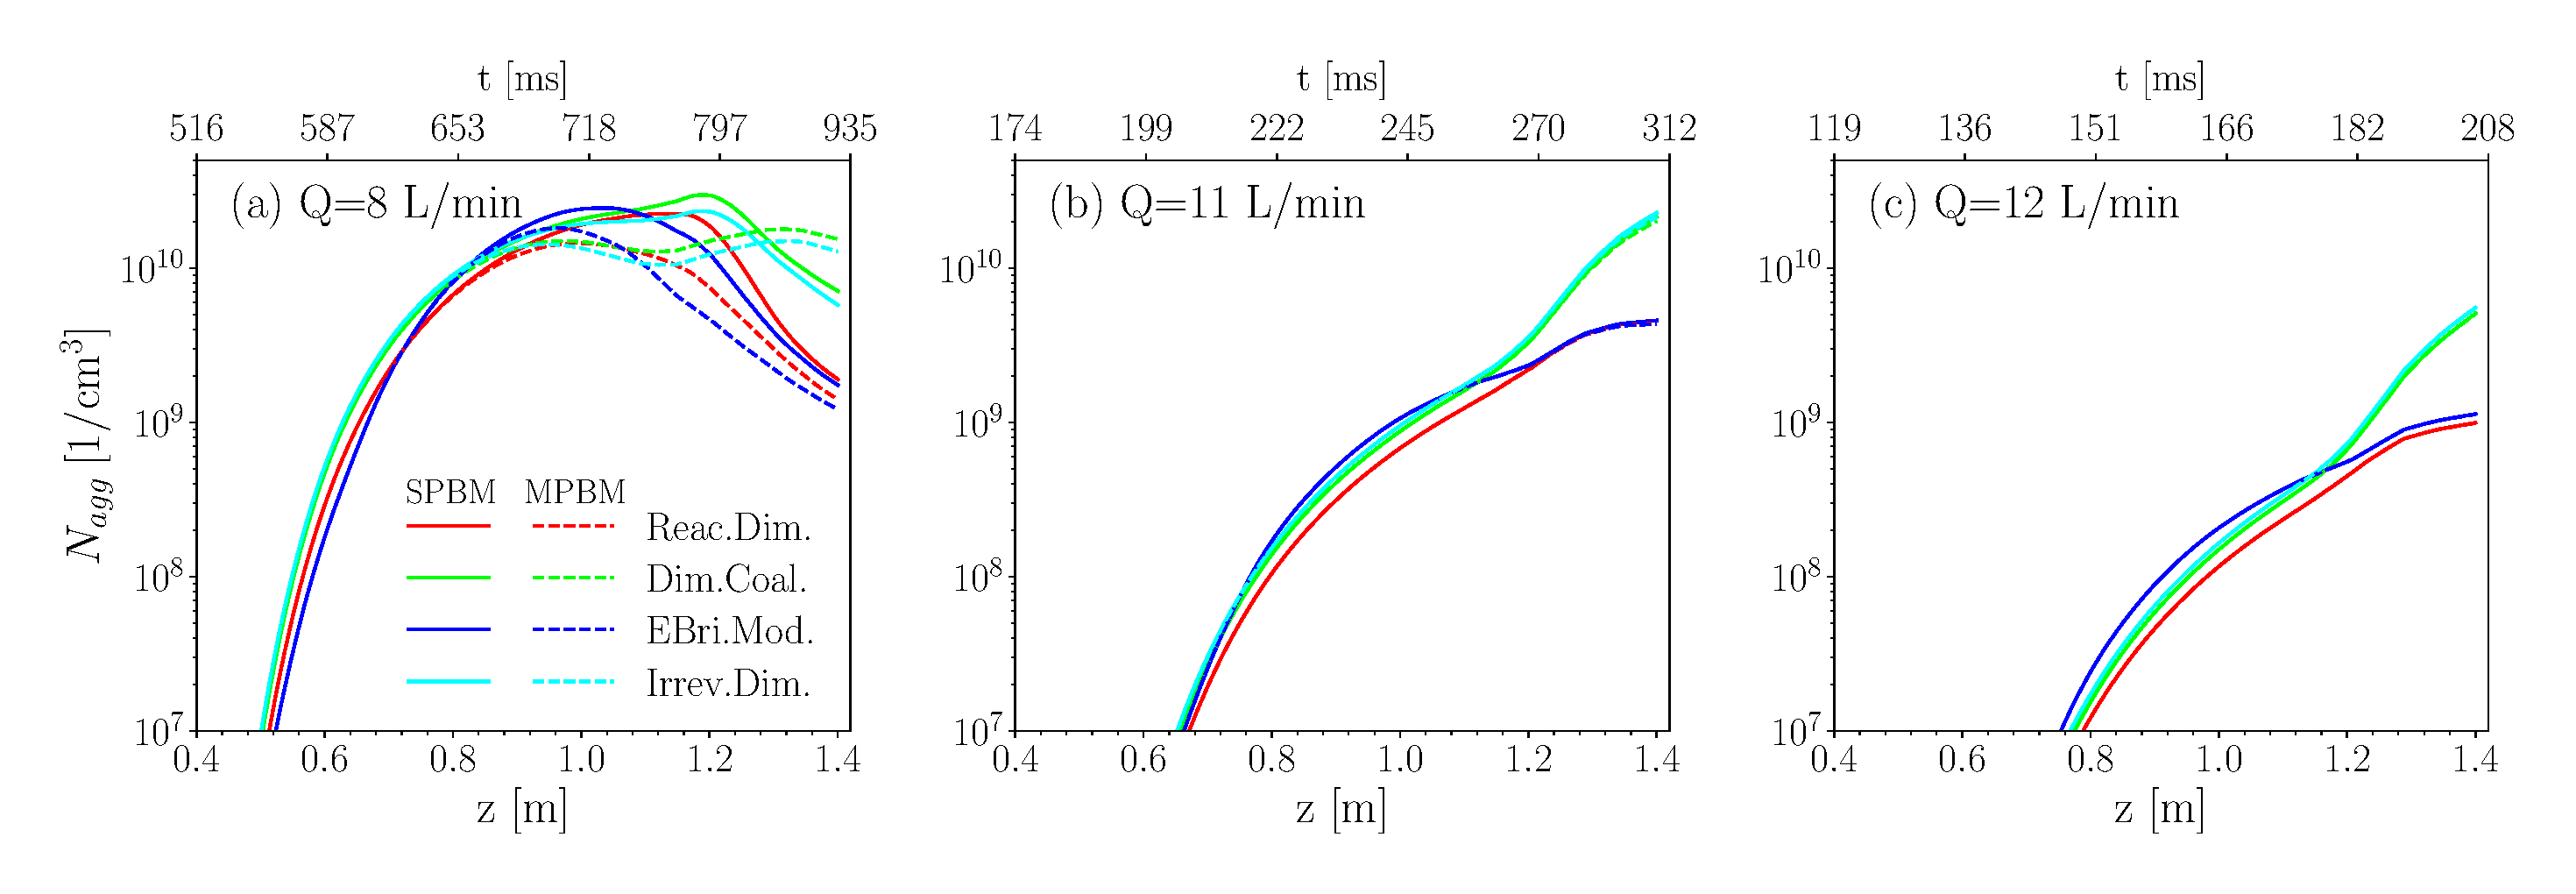
\includegraphics[width=1\textwidth]{Figures/Results/PFR/N_agg_pdynamiceffect.pdf}
	\caption{The effect of particle dynamics on total number of agglomerates, $N_{agg}$ along the PFR for Q=8 (a), 11 (b), and 12 L/min (c) using different inception models.}
	\label{fig:pfr_Nagg_pdynamicseffect} 
\end{figure}

Fig.\ref{fig:pfr_Nagg_pdynamicseffect} compares $N_{agg}$ predicted by the sectional (solid) and monodisperse (dashed) population balance model using different inception models. For Q=8 L/min, $N_{agg}$ is the same for both particle dynamics model up to 0.8 where soot inception has dominant effect on total number of agglomerates compared to coagulation, but after that monodispere model predicts stronger collision rate leading to smaller number of agglomerates after the peak. When the monodisperse model is used with Dimer Coalescence and Irreversible Dimerization, the underprediction of $N_{agg}$ is followed by a secondary increase that exceed the prediction of the sectional model. This behavior can be better understood by looking at inception fluxes shown in Fig.~\ref{fig:pfr_Iinc_pdynamicseffect} that are the same for both particle dynamics models. These two inception models continue to produce new particles in the cooling region of the reactor near the end due to their weak temperature dependence. This causes a significant increase in $N_{agg}$ for both particle dynamics models. The peak number concentration of agglomerates is larger for the sectional model resulting in a stronger decay near the end of the reactor.


\begin{figure}[H]
	\centering
	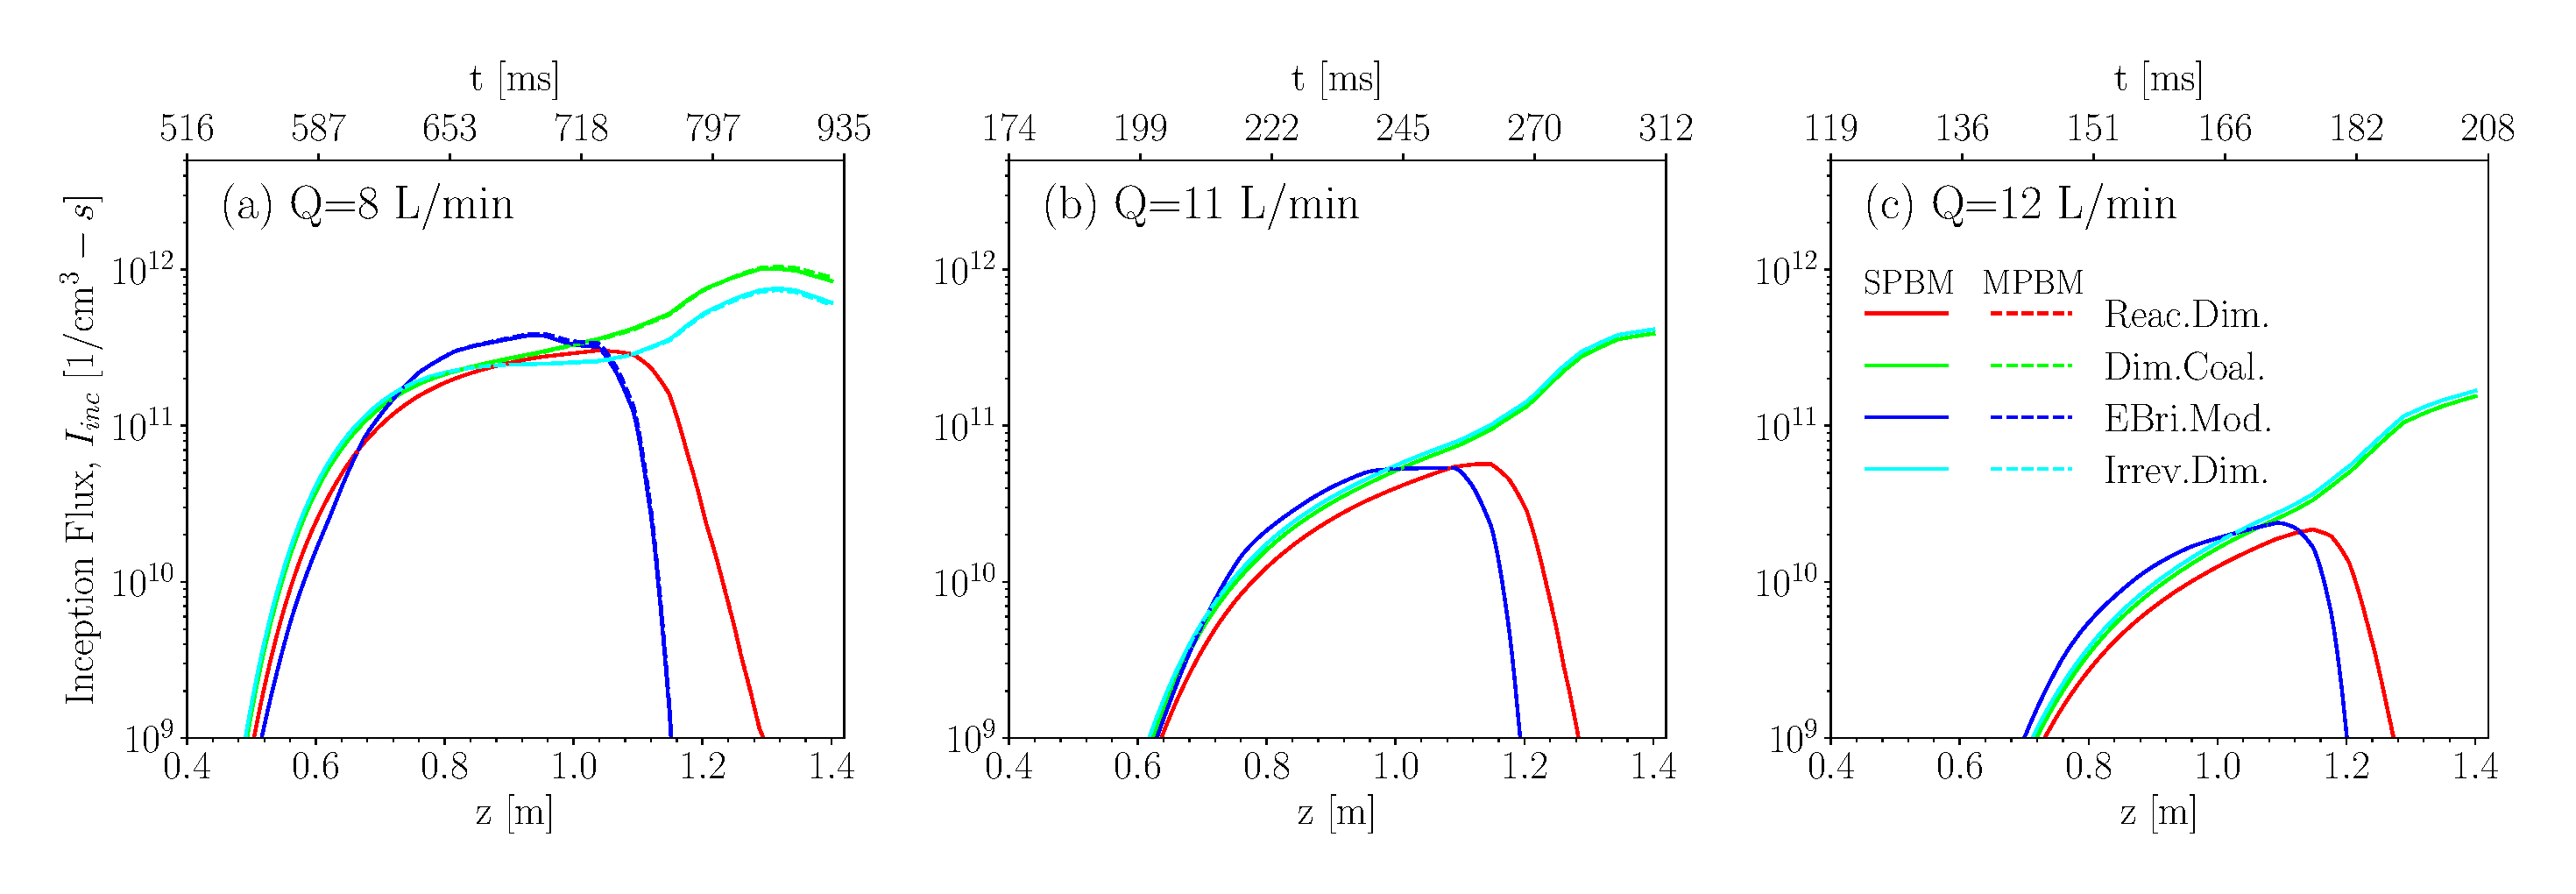
\includegraphics[width=1\textwidth]{Figures/Results/PFR/inception_pdynamiceffect.pdf}
	\caption{The effect of particle dynamics on inception flux, $I_{inc}$ along the PFR for Q=8.5 (a), 11 (b), and 12 L/min (c) using different inception models in a 0.6\%$\mathrm{C_2H_4}$ pryolysis in a flow reactor~\citep{mei2019quantitative}}
	\label{fig:pfr_Iinc_pdynamicseffect} 
\end{figure}



\begin{figure}[H]
	\centering
	\begin{subfigure}[t]{0.4\textwidth}
		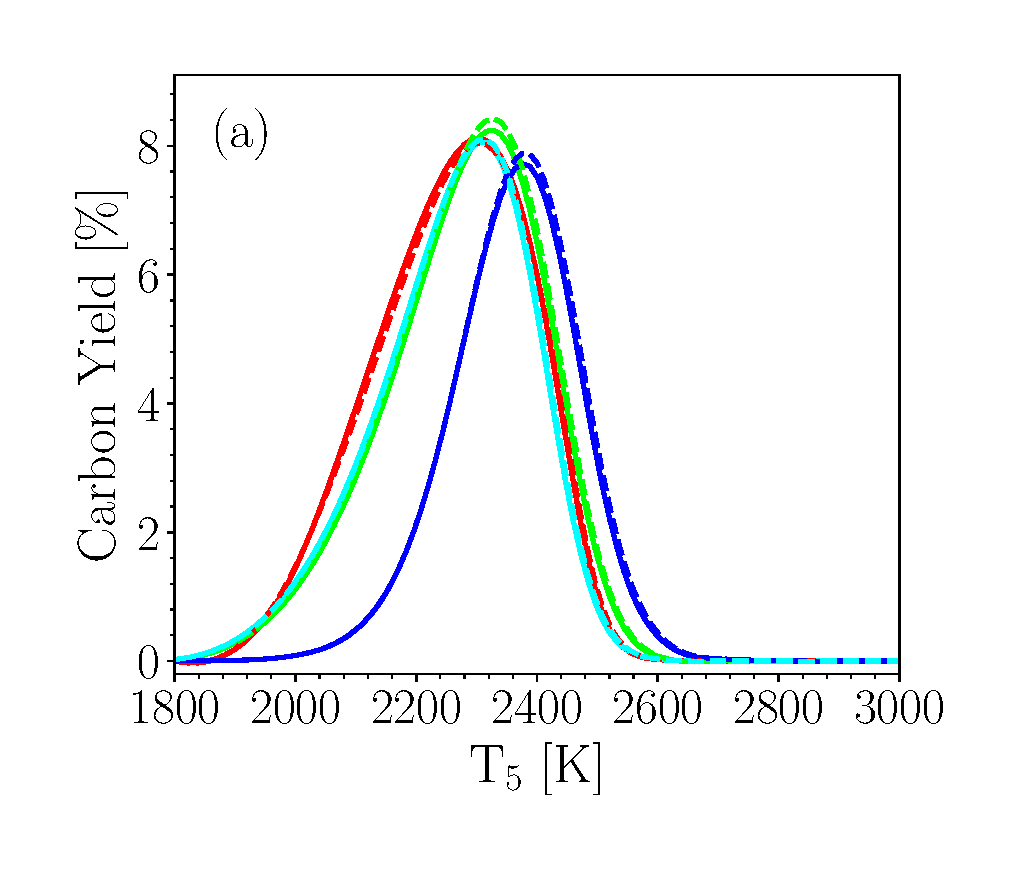
\includegraphics[width=1\textwidth]{Figures/Results/Shocktube/Agafonov2016_cvr/carbon_yield_pdynamiceffect.pdf}
	\end{subfigure}
	\begin{subfigure}[t]{0.435\textwidth}
		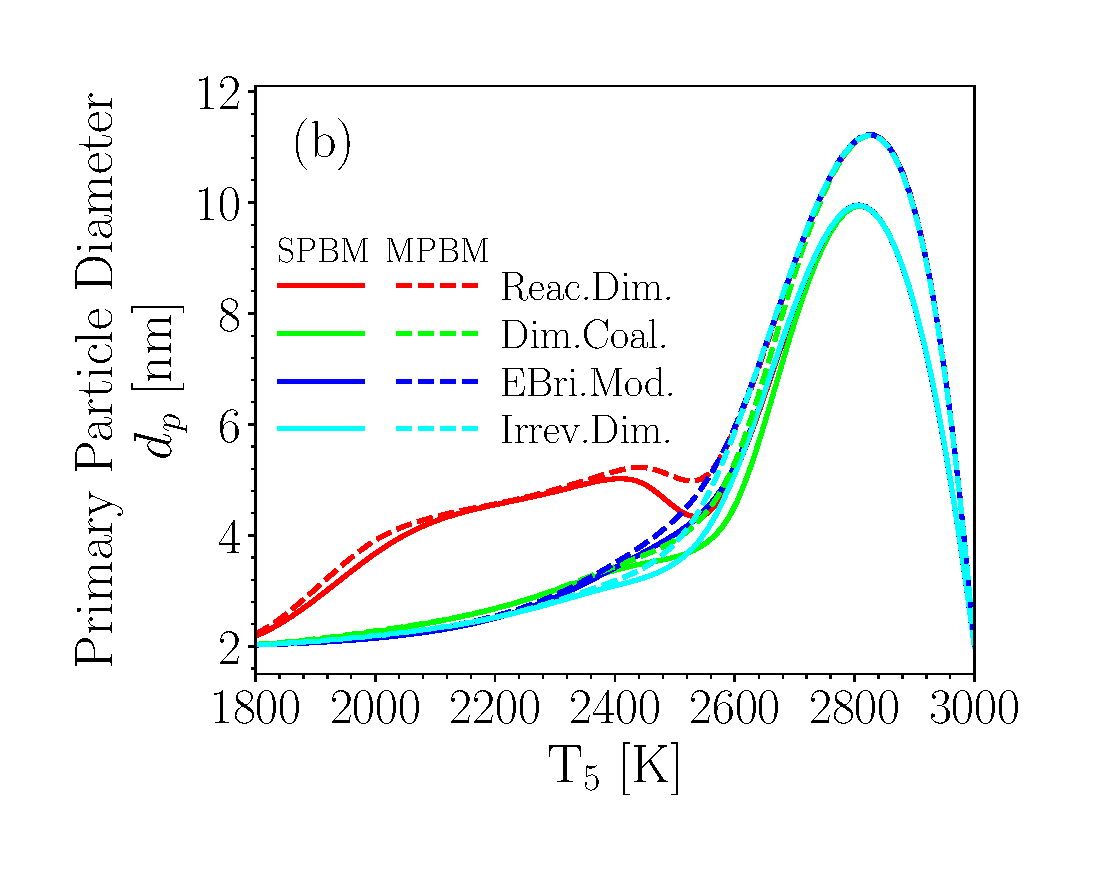
\includegraphics[width=1\textwidth]{Figures/Results/Shocktube/Agafonov2016_cvr/d_p_pdynamiceffect.pdf}
	\end{subfigure}
	\caption{The effect of particle dynamics model on soot carbon yield (a) and mean primary particle diameter, $d_p$ (b) at t=1.5 ms over 1800$<T_5<$3000 K during 5\%$\mathrm{CH_4}$ pyrolysis~\citep{agafonov2016unified}}
	\label{fig:shockagof_pdynamiceffect} 
\end{figure}